\chapter{Analysis}
Before we move to the nuts and bolts of AlphaZero and our concrete implementation, we should establish a general understanding of the problem. That includes building the necessary theoretical background in artificial intelligence in general, as well as insight into the specialized knowledge such as deep reinforcement learning in particular.

\section{Artificial intelligence}
Since the late 1960s, many artificial intelligence researchers presumed that there are no general principles to be discovered, that intelligence is instead due to the possession of a vast number of special purpose tricks, procedures, and heuristics. It was sometimes said that if we could just get enough relevant facts into a machine, say one million, or one billion, then it would become intelligent. Methods based on general principles, such as search or learning, were characterized as “weak methods,” whereas those based on specific knowledge were called “strong methods.” This view is uncommon today. From our point of view, it was premature: too little effort had been put into the search for general principles to conclude that there were none. Modern artificial intelligence now includes much research looking for general principles of learning, search, and decision making. It is not clear how far back the pendulum will swing, but reinforcement learning research is certainly part of the swing back toward simpler and fewer general principles of artificial intelligence.

% explain some of the history of AI:
% - what does it mean
% - little bit of history: focus on symbolic vs subsymbolic

\subsection{Rational agent}
Stemming from the latin word \textit{agere} meaning "to act", an agent is something that acts. As we expect our agent to take sensible or intelligent actions we further qualify this definition by calling it rational. This means that it acts so as "to achieve the best outcome or, when there is uncertainty, the best expected outcome". \cite[p. 36]{russell_artificial_2021}

The agent exists in an environment which it perceives through sensors and it takes actions through its actuators. We refer to the content of the sensor's output for one observation as \textit{percept}. The cat uses eyes, ears and other organs to perceive the world and its legs, claws and so on to interact with the world. An autonomous car might use radar and cameras for acquiring information and steering and motors for navigation.

Internally our agent might have some built-in knowledge about the world, such as rules on how the environment works. The \textit{agent function} takes the entire history of percepts observed and this built-in knowledge and maps it to an action. A concrete implementation of this abstract function is called \textit{agent program}. The agent program might just be a simple tabular mapping from percepts to actions or could use a complex algorithm with an additional model.

\subsection{Task environment}

As we are trying to build an agent that tries to achieve some specified goal, we can consider our environment as a problem or \textit{task} our agent tries to solve. Putting together both agent and the environment we see a loop of observing,  deliberating and finally taking an action as depicted in figure \ref{agent_environment_loop}.

\begin{figure}
    \centering
    % \includesvg[height=7cm]{agent_environment_loop.svg}
    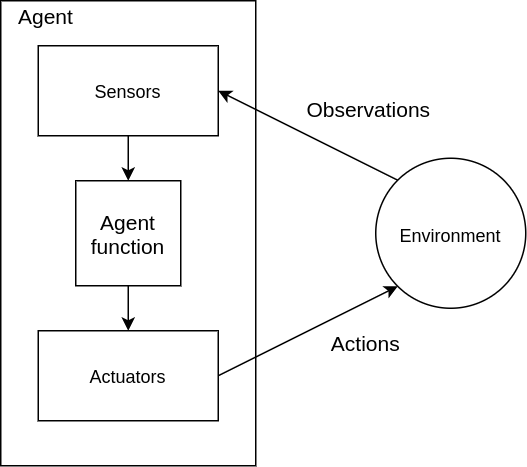
\includegraphics[height=7cm, keepaspectratio]{agent_environment_loop.png}
    \caption{The agent-environment interaction loop}
    \label{agent_environment_loop}
\end{figure}

\section{Environment}
Now that we have a general understanding of agents and environments, we can use this knowledge to have a closer look at Abalone. It is a fairly new game that was devised in 1987 by Michel Lalet and Laurent Lévi. Nevertheless, with more than four million global sales it has established itself as a classic game \cite{noauthor_abalone_2020}. Abalone is a two-player game consisting of a hexagonal board with 61 fields and 14 marbles for black and white respectively.

\subsection{Abalone rules}
The goal of the game is to push six of the opponent's marbles off the playing field. The game's starting position is depicted in figure \ref{basics} (a). One, two, or three adjacent marbles (of the player's own color) may be moved in any of the six possible directions during a player's turn. We differentiate between broadside or "side-step" moves and "in-line" moves, depending on how the chain of marbles moves relative to its direction, which is shown in figure \ref{basics} (b) and (c).

\begin{figure}[!h]
    \centering
    \subfloat[Starting position]{
        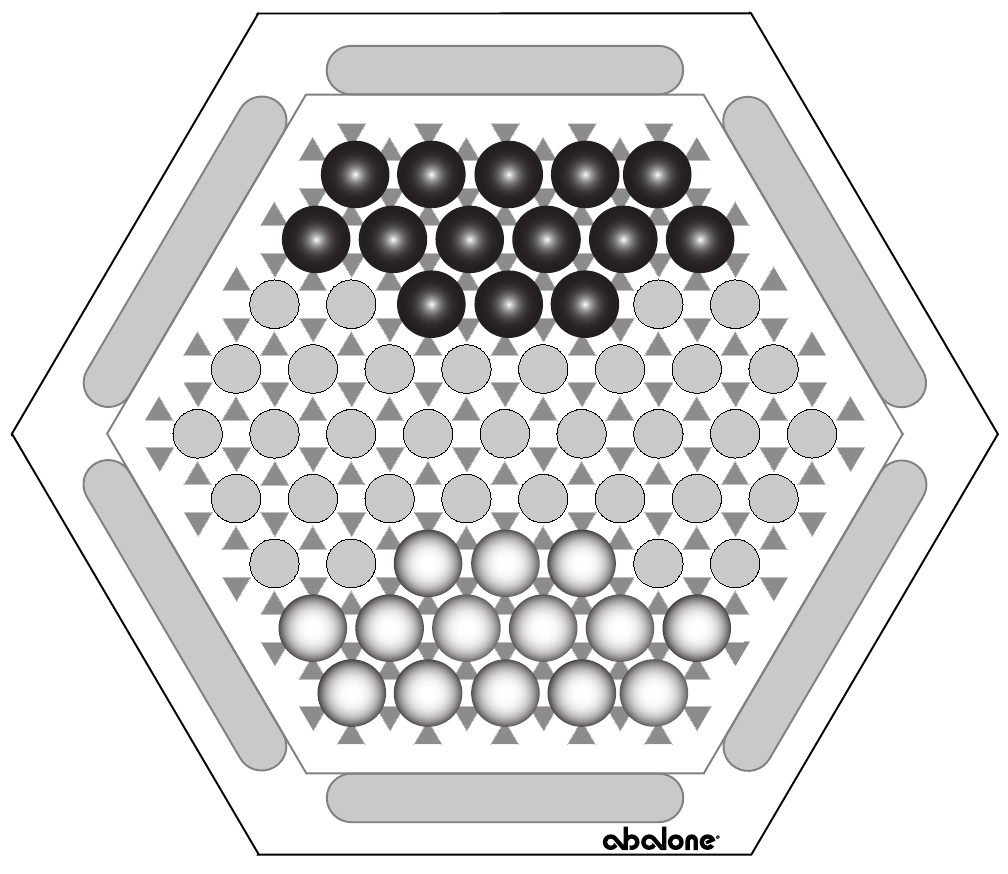
\includegraphics[width=3cm, keepaspectratio]{rules_starting_position.png}
    }
    \hfill
    \subfloat["In-line" moves]{
        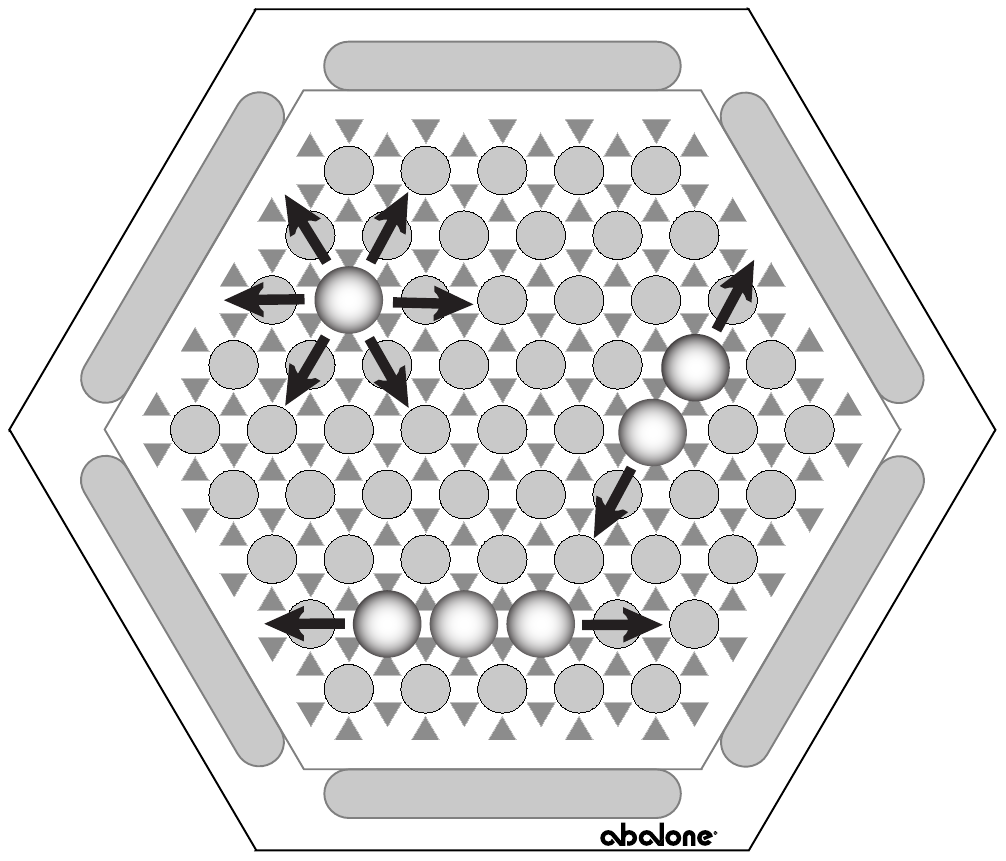
\includegraphics[width=3cm, keepaspectratio]{rules_inline_move.png}
    }
    \hfill
    \subfloat["Side-step" moves]{
        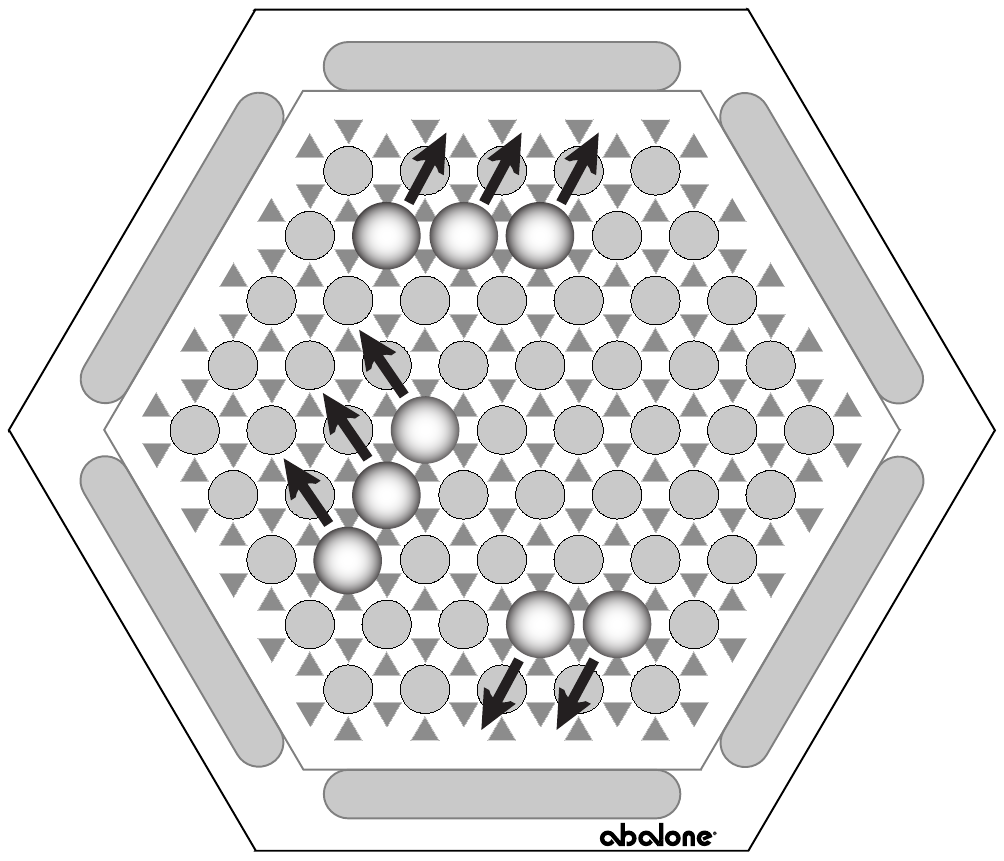
\includegraphics[width=3cm, keepaspectratio]{rules_side_step_move.png}
    }
    \caption{Basic moves \cite{abalone_sa_abalone_nodate}}
    \label{basics}
\end{figure}

A move pushing the opponent's marbles is called "sumito" and comes in three variations, as shown by figure \ref{sumito}. Essentially, the player has to push with superior numbers and the opponent's marbles can not be blocked. This is the game mechanic that allows for pushing the marbles out of the game and winning.

\begin{figure}[!h]
    \centering
    \subfloat["2-push-1" sumito]{
        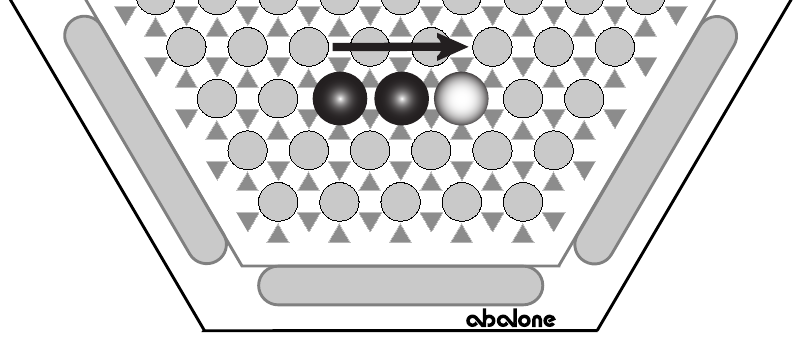
\includegraphics[width=3cm, keepaspectratio]{rules_2-push-1_sumito.png}
    }
    \hfill
    \subfloat["3-push-1" sumito]{
        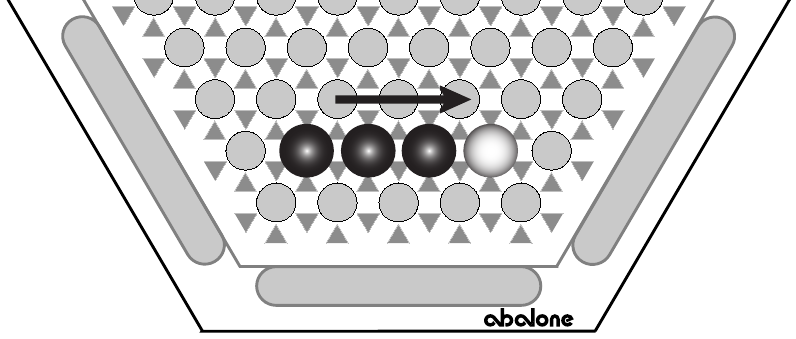
\includegraphics[width=3cm, keepaspectratio]{rules_3-push-1_sumito.png}
    }
    \hfill
    \subfloat["3-push-2" sumito]{
        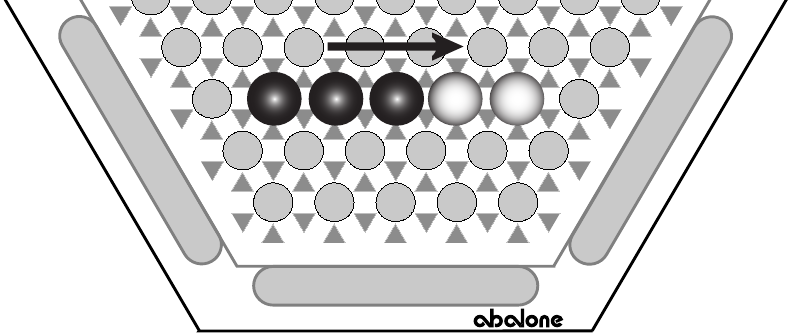
\includegraphics[width=3cm, keepaspectratio]{rules_3-push-2_sumito.png}
    }
    \caption{Sumito positions allow pushing the opponent's marbles \cite{abalone_sa_abalone_nodate}}
    \label{sumito}
\end{figure}

\subsection{PEAS and task properties}
Based on the PEAS framework we can specify Abalone as a task environment and show the key components for the implementation of our agent. \cite[p.107]{russell_artificial_2021}

\begin{description}
    \item[Performance measure] Win/loss, number of moves, time to deliberate
    \item[Environment] Digital playing board
    \item[Actuators] Move marbles, display text to CLI
    \item[Sensors] Position of marbles
\end{description}

There are a few categorizations that are extremely helpful for narrowing down potential applicability of different classes of algorithms. A key property is the observability of the environment. If the environment is \textit{fully observable}, the sensors detect all the information that is in any way relevant for taking an action. Conversely if not all information can be observed we call it \textit{partial observability}. For example in poker the other players' cards and the upcoming cards cannot be seen but are highly relevant to the agent's actions. As the current board state of Abalone fully comprises all information necessary to make a move, we can classify it as fully observable.

The values of the state of the environment and time can be categorized into discrete and continuous. The autonomous vehicle for instance is dealing with continuous time and also continuous states. The speeds of the car take a smooth range of real values and time can be meaningfully split into increasingly small intervals. However, Abalone is entirely discrete. The set of all states is a finite collection of all (legal) permutations of the board and the marbles. Time progresses on the basis of turns.

The actions that the agents take might also be \textit{non-deterministic}. When dealing with systems of high complexity the next state might not only depend on the previous state and the action taken. There might be other car drivers taking unexpected actions or a comet hitting our car. In Abalone none of these issues arise as it is deterministic.

Further expanding on the passage of time we have to take into account if actions have consequences for future states. If each combination of percept and action is independent of each other we call it \textit{episodic} and \textit{sequential} otherwise. If we had to classify a production line of circuit boards as either defective or functional, it would be an episodic environment. The classification of an individual board does not matter for the next one. In the case of Abalone, moves taken have long drawn out consequences for later stages of the game.

Another aspect of time is whether the environment changes while the agent takes time to deliberate on the next move. In a \textit{dynamic} environment like the autonomous vehicle operates in, the environment changes continuously. By the time the car decides whether to go right, to avoid collision with a wall, this decision might have already become obsolete. As any turn-based game, Abalone is a \textit{static} environment, as the board only changes after a move is made.

Lastly, an additional dimension to consider is the number of agents involved. The classification of circuit boards only involves one agent whereas Abalone is a \textit{multi-agent} environment. We also have to distinguish whether those multiple agents compete for the performance measure. In Abalone, one player's win is the other player's loss. In contrast, the other vehicles apart from our autonomous vehicle all profit when it avoids a collision and vice versa. Therefore, they cooperate.

Summing this up \textbf{Abalone is a fully observable, deterministic, two-agent, competitive, sequential, static and discrete environment}. Another popular term for this type of environment is a \textit{perfect information zero-sum game}.

\subsection{Abalone complexity}

As Abalone has a finite amount of discrete states, we can make precise statements about its complexity, which can be described in two relevant dimensions.

\paragraph{State space complexity}
The state space is the set of all possible states the environment can be in.\cite[p. 150]{russell_artificial_2021} For Abalone this means we have to consider all possible board configurations with different numbers of marbles present. Additionally, we would have to remove duplicates that arise from the symmetries of the board. In the case of abalone we have 6 rotations and 6 axes we can mirror the board on. The following formula gives us a good upper bound:

$$
    \sum_{k=8}^{14}\sum_{m=9}^{14}\frac{61!}{k!(61-k)!}\times\frac{(61-k)!}{m!((61-k)-m)!}
$$

\paragraph{Game tree complexity} The game tree defines all transitions between board positions (nodes) through moves (edges). The \textit{search tree} is potentially a subset of the game tree, if not all paths are visited. In the case of Abalone the game tree is unbound and has an infinite height as actions might be taken repeatedly forming loops. To get a measure of the complexity the number of nodes in a tree is given by:

$$
    b^d
$$

First we consider the branching factor $ b $, or the number of possible moves for any given state. We can only approximate this, as this number greatly varies between different states. On average abalone has $ b = 60 $ possible moves per state as measured in figure \ref{branching_factor}. The depth $ d $ of the tree depends on the number of turns per game. Looking at the average again a game takes in the region of $ d = 87 $ turns, giving us a total of $60^{87}$ nodes. To be precise this is the complexity of an average search tree not the game tree, as mentioned above. \cite{lemmens_constructing_2005}

\begin{figure}
    \centering
    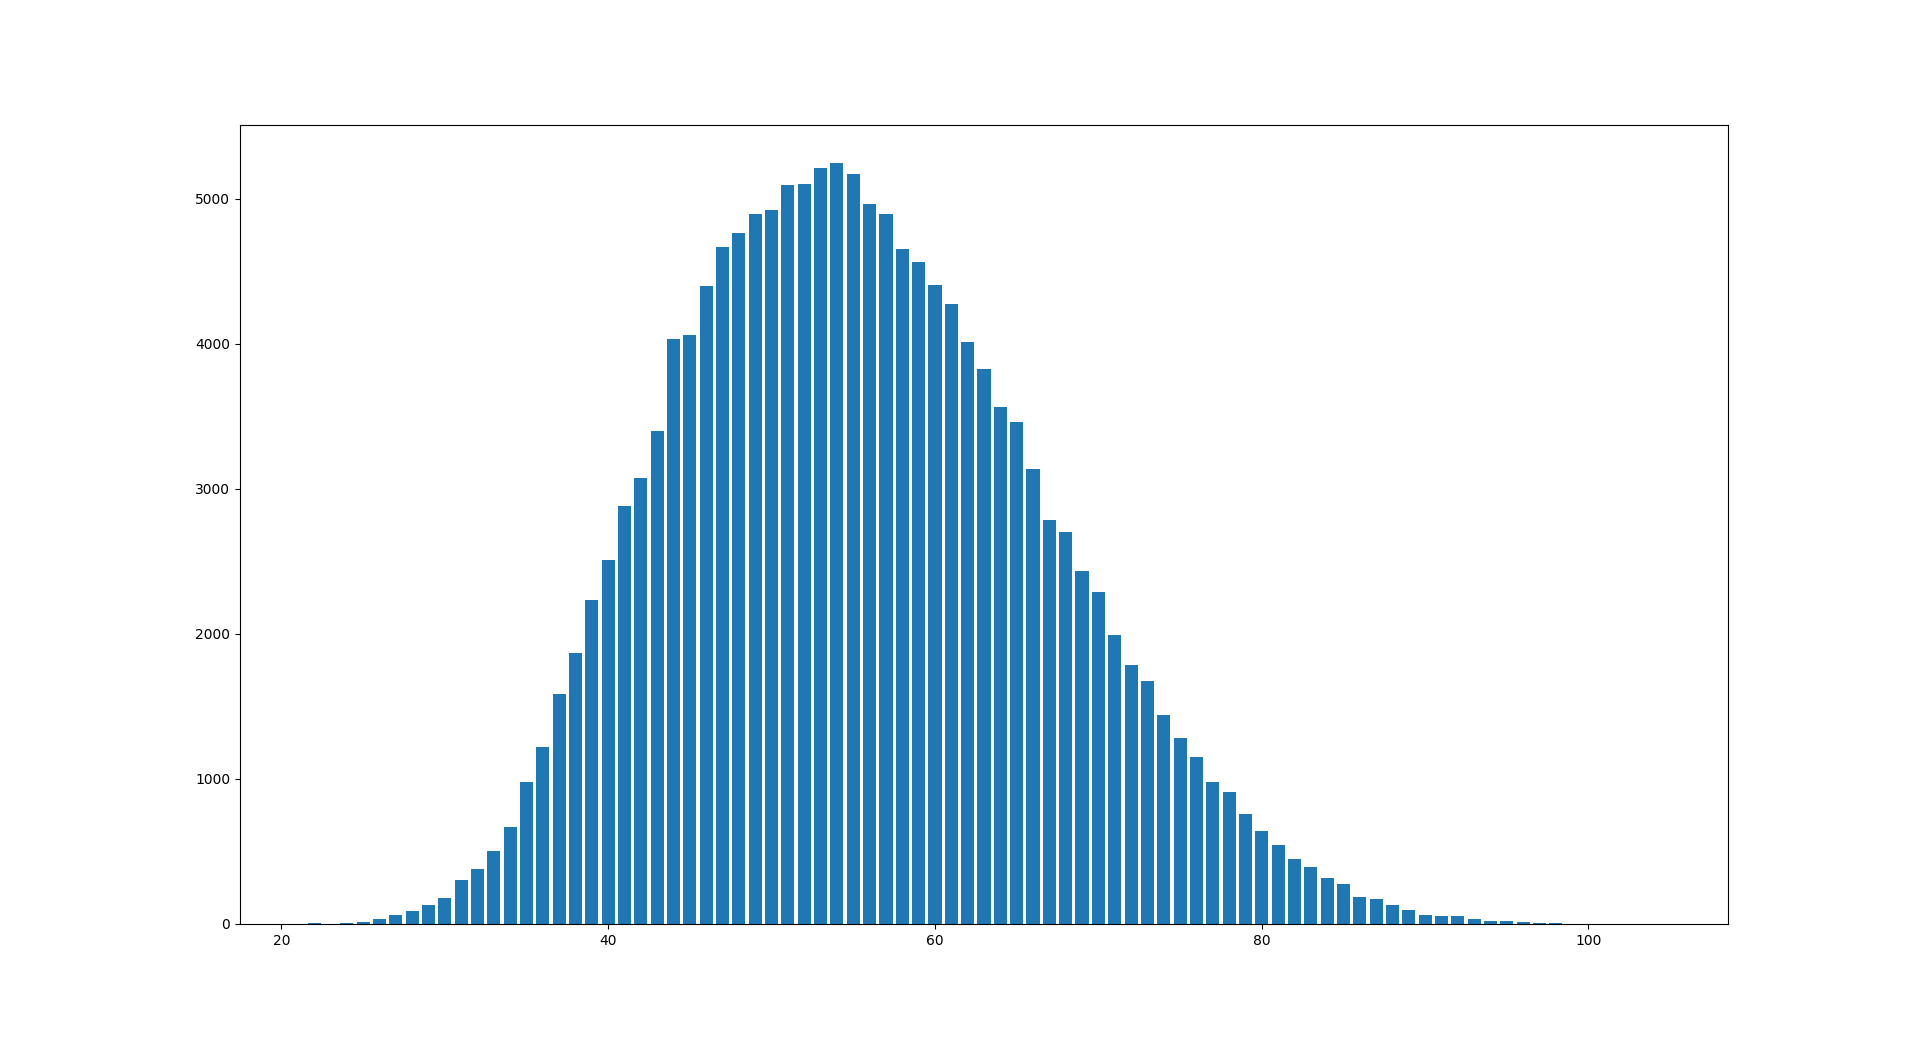
\includegraphics[width=7cm, keepaspectratio]{distribution_of_moves.png}
    \caption{Counts of moves available for random for random player in 5 games}
    \label{branching_factor}
\end{figure}

As those numbers in isolation are hard to grasp it is useful to put Abalone's complexity in relation with other popular games. Its state space complexity is on the same level as Reversi, whilst its game tree surpasses chess in complexity (c.f. table \ref{complexity_table})

\begin{table}
    \begin{center}
        \begin{tabular}{ | c | c | c | }
            \hline
            Game        & state-space complexity (log) & game-tree complexity (log) \\
            \hline
            Tic-tac-toe & 3                            & 5                          \\
            \hline
            Reversi     & 28                           & 58                         \\
            \hline
            Chess       & 46                           & 123                        \\
            \hline
            Abalone     & 24                           & 154                        \\
            \hline
            Go          & 172                          & 360                        \\
            \hline
        \end{tabular}
    \end{center}
    \caption{Abalone in comparison with other games \cite{chorus_implementing_2009}}
    \label{complexity_table}
\end{table}


\section{Classic agent}
Now that we have an intricate understanding of the environment for our agent we have also narrowed down the choice of algorithms we can employ. In general, perfect information games can be solved by adversarial search algorithms. That means in theory we can find the optimal solution by traversing the entire game tree to terminal states (game ending state). The theory behind this type of agent was already laid out as early as 1945 by Konrad Zuse's program generating legal chess moves \cite{knuth_early_1980}, but was described most comprehensively by Claude Shannon in 1950 in "programming a Computer for Playing Chess". \cite{shannon_xxii_1950}

\subsection{Minimax algorithm}
Minimax assumes two roles: The minimizer and the maximizer. We start the search from the current board state as the role of the maximizer and then alternate between the two. The result of the minimax search gives us the maximum utility for the given state, assuming both players behave optimally. Let us define the functions
\begin{itemize}
    \item $\text{utility(s, p)}$ returns the utility or the payoff for the terminal state $s$ seen from the perspective of player $p$. In the case of abalone this might be -1, 0 and 1 for a loss, draw and a win.
    \item $\text{is-terminal(s)}$ returns whether the given state $s$ is a terminal state or not
    \item $\text{to-move}(s)$ returns the current player for the state $s$
    \item $\text{result}(s, a)$ returns the resulting state if in state $s$ and taking action $a$
\end{itemize}
such that we can define minimax recursively as:
$$
    \text{minimax}(s) =
    \begin{cases}
        \text{utility}(s, max)                                                & \text{is-terminal}(s)    \\
        \text{max}_{a\in\text{actions}(s)}\text{minimax}(\text{result}(s, a)) & \text{to-move}(s) == max \\
        \text{min}_{a\in\text{actions}(s)}\text{minimax}(\text{result}(s, a)) & \text{to-move}(s) == min \\
    \end{cases}
$$

Putting this together we can see in figure \ref{minimax} a graphical representation of the search tree for an abstract example. The algorithm traverses down to a leaf node, evaluates its utility and passes the value back up to the parent node. Depending on whether it is a minimizer or a maximizer it chooses the smallest or the largest value passed up by its children. This value again is passed up to the parent until we reach the parent node which is always a maximizer, yielding us the maximum utility we can achieve given our opponent plays optimally.

\begin{figure}
    \centering
    % \includesvg[height=7cm]{minimax.svg}
    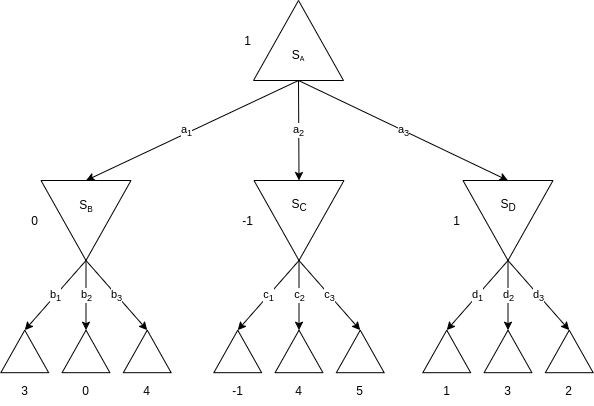
\includegraphics[height=7cm, keepaspectratio]{minimax.png}
    \caption{Minimax for a small search tree, resulting in an utility value of 1}
    \label{minimax}
\end{figure}

\subsection{Heuristic functions}
As the number of nodes of the game tree gets very large, the search on the tree usually does not reach terminal leaves that indicate a clear loss or win. Our computational resources will get exhausted first. For example minimax has already visited $ 60 ^ 4 = 1.2960.000 $ nodes at a depth of $ d = 4 $ in the case of an average Abalone game.

Therefore, one has to limit the search to a computationally feasible depth and evaluate the intermediary result of a given transposition based on a so-called \textit{heuristic function}. This function replaces our previous $ utility(s) $ for terminal states and is based on human knowledge. The function should give precise feedback on the quality of a state from the perspective of the given player. A sensible function for Abalone might be a linear combination in the form of:

$ h(s) = \omega_0f_0(s) + ... + \omega_nf_n(s) $

With functions $ f_i $ calculating different values such as

\begin{itemize}
    \item Adjacency: As a majority of marbles is required to push the opponent's marbles and conversely an equal amount of marbles is needed to avoid being pushed, it can be assumed that keeping one's marbles grouped together is a good move.
    \item Distance to center: Marbles that are close to the brink of the board put them into danger of being attacked, wherefore it is generally good to place all of the marbles into the center of the board. For each player's marbles we measure their distance from the center of the board as the smallest amount of moves it would take to reach the center (Manhattan distance).
    \item Win and loss: As a more definitive measure we can indicate whether the current state is a terminal state and hence a winning or losing state.
    \item Etc.
\end{itemize}

By applying different weights $ \omega_i $ to the functions $ f_i $ we essentially give incentives to the agent to prioritize certain behavior. If the win or loss function returns a value of either -1 or +1, we might combine it with a weight of 10.000 to make sure we choose winning states and avoid losing states above all. Armed with this heuristic function we can find good moves with minimax search even in highly complex state spaces.

However, the problem with heuristic is we need expert knowledge and a lot of empirical testing to find a suitable heuristic. In some cases like with Go, such a heuristic function might not be competitive with even moderate human players. In other cases such as chess this strategy is very powerful. As mentioned in the introduction IBM's Deep Blue could beat the world's best player Gary Kasparov with this heuristic based adversarial search.

\subsection{Alpha-beta pruning}
We can further improve minimax search markedly by using Alpha-beta-pruning. This method tries to eliminate unnecessary traversals down the search tree. In the best case, this leads to a reduction of nodes from $ O(b^d) $ to $ O(\sqrt{b^d}) $.

\begin{figure}
    \centering
    % \includesvg[height=7cm]{alpha_beta_pruning.svg}
    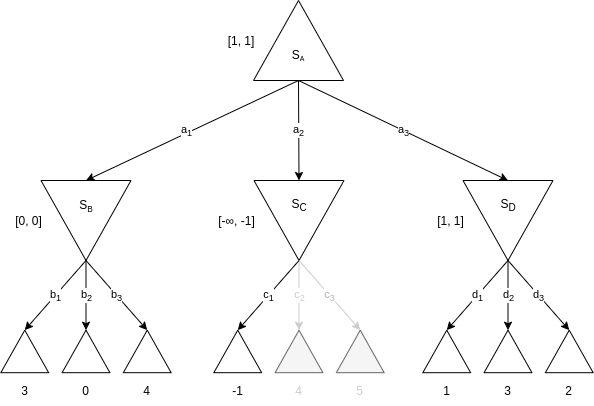
\includegraphics[height=7cm, keepaspectratio]{alpha_beta_pruning.png}
    \caption{Our previous example but with alpha beta pruning applied. The grayed out nodes indicate, that these in fact could be pruned from the tree}
    \label{alpha_beta_pruning}
\end{figure}

The order in which we visit nodes in minimax is similar to a graph traversal with depth first search, meaning we descend down until we find a leaf node. This gives us information about the utility of that node and, consequently, part of the tree. Going up the tree we keep an alpha value for the minimum value the maximizer will receive and a beta value for the maximum value the minimizer will achieve. For instance this lets us know if the minimizer already can choose a move worse than what we can achieve with another move, we do not descend further $ (\alpha > \beta) $.

Looking at the example in figure \ref{alpha_beta_pruning} will help us illustrate this principle. Our search revealed that choosing move $ a_1 $ will yield us an utility of at least 0. Traversing down move $ a_2 $ the first leaf has a utility of -1. Hence, the minimizer will choose a move that is at most -1 which is already worse than the utility of 0. We need not look further at this part of the tree.

The example also shows us an important prerequisite for this method to work. The order in which we expand which node matters decides how many nodes we can prune. Had we visited move $ c_3 $ and $ c_2 $ first, pruning wouldn't have been possible. The best case of $ O(\sqrt{b^d}) $ is entirely dependent on this ordering. We could find different ways of ranking the moves:

\begin{itemize}
    \item \textit{Killer move heuristic} prioritizes that are usually undoubtedly good like taking a marble in Abalone.
    \item \textit{Iterative deepening} Performs a minimax search only to a depth of one and uses the resulting values to rank the moves. Then searching one level deeper we use this ranking for ordering the moves. Even though there is a lot of redundancy, we make up for this more than enough by pruning much more effectively.
\end{itemize}

Other improvements to the procedure are thinkable as well. Once we perform a search for a certain state, we can store the resulting utility. If we encounter this position again, because of a different permutation of the move sequence (transposition), we can just look up the state utility in the \textit{transposition table}.

Combined with alpha beta pruning, the minimax algorithm is a very efficient way of finding the optimal utility in an adversarial search situation. However, as mentioned before in most games we cannot use the utility of terminal states, because the search tree grows too quickly. By optimizing for a heuristic function the quality of play solely depends on this function. For games such as Chess or Abalone minimax has been very successful, because humans could devise meaningful heuristic functions. For chess the engine stockfish has been the most successful computer player for a long time and is based on this algorithm (and many optimizations). \cite{noauthor_stockfish_2021, noauthor_stockfish_nodate} In Abalone there are multiple implementations, the most successful has been ABA-PRO by Tino Werner from 2002 \cite{aichholzer_algorithmic_2002} which has been the reference for other algorithms such as Abalearn \cite{campos_abalearn_2003}. A more recent publication by Papadopoulos et. al. claimed to have devised a more successful player than Werner. \cite{papadopoulos_exploring_2012} This was confirmed in a very recent reimplementation thesis by Michiel Verloop \cite{verloop_critical_nodate}. This reimplementation in Java \cite{verloop_abaloneai_nodate} is also the reference for later benchmarks.

\subsection{Monte Carlo Tree Search}
For games like Go we cannot find powerful heuristic functions, which makes the previous approach of minimax not a viable option. In addition, the initial position of a 19x19 Go board is 361 decreasing only by one for each stone placed. A method proposed in 2006 by Coulom \cite{coulom_efficient_2007} called Monte Carlo Tree search. The main idea is to use simulations or \textit{rollouts} to gain information on the quality of a state. To manage the complexity of the search tree more effectively the algorithm is \textit{selective} in which parts of the tree are \textit{expanded}. This ensures that resources are not wasted on unpromising moves.

In its purest form the simulations are performed randomly, meaning we take a state or node to be investigated and let two random players take turns until a terminal state is reached. Kocsis and Szepesvári \cite{kocsis_bandit_2006} showed that it does in fact converge to optimal play. For games like Abalone with a high branching factor we need a large number of simulations to get any meaningful information from the simulations, so we might use a \textit{rollout policy} instead. This policy guides the moves taken in the simulation towards better moves. This might be as simple as favoring capturing moves or as we will see later neural networks.

The algorithm can be structured into four stages:

\paragraph{Selection} is the process of deciding which node to consider next. We start at the root node and select a node until we reach a leaf node. This is the selected Node. We could select the nodes according to some stationary distribution or we could use the information that we gain over time.

\paragraph{Expansion} is the step in which we expand the selected node by appending a fresh child node.

\paragraph{Simulation} is as described before the step in which we perform a simulation with our rollout policy starting from the state of the newly generated child node.

\paragraph{Back-propagation} is the last step. We take the result of the simulation (utility) and write it to the node and parent nodes above until we reach the root node. Each node updates its cumulative utility $U(n)$ and the number of times it was visited $N(n)$.

The more we repeated this cycle, the more certainty we gained about the optimal move to take.

\begin{figure}
    \centering
    % \includesvg[height=7cm]{minimax.svg}
    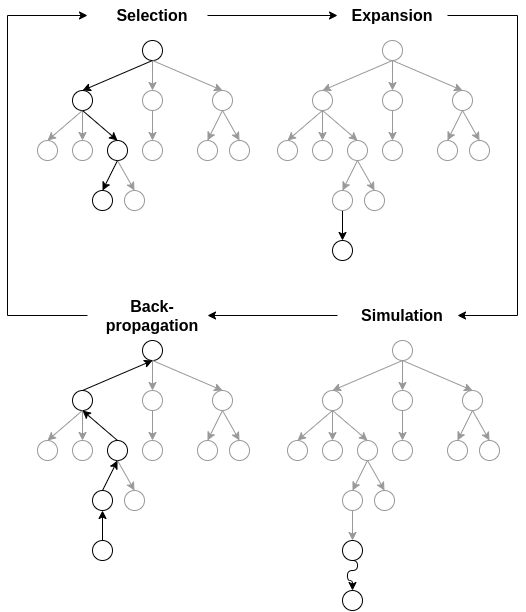
\includegraphics[height=9cm, keepaspectratio]{monte_carlo_tree_search.png}
    \caption{Monte Carlo tree search stages \cite{noauthor_fig_nodate}}
    \label{monte_carlo_tree_search}
\end{figure}

The inception of MCTS led to significant improvements in performance of game-playing agents in the Game of Go. The algorithm "Crazy Stone" from Coulom won the 10th KGS computer-Go tournament against competitors such as Indigo \cite{bouzy_associating_2006}. To select the next node he estimated the probability of that move being better than the current best move. We order the moves by their current estimated value $ \mu_i $ and calculate the corresponding variance $ \sigma_{i}^{2} $ getting the ordering of $ \mu_0 > \mu_1 > ... > \mu_N $. Selection of a move is proportional to:

$$
    u_i = exp\left(-2.4\frac{\mu_0 - \mu_i}{\sqrt{2(\sigma_{0}^{2} + \sigma_{i}^{2})}}\right) + \epsilon_i
$$

The Term $ \epsilon_i $ ensures that the probability of selection never goes to zero as defined by $ \epsilon_i = \frac{0.1 + 2^{-i} + a_i}{N} $. The resulting distribution is similar to the Gaussian distribution and the Boltzman equations \cite{coulom_efficient_2007}

Another idea for selection is the UCB1 formula \cite{auer_finite-time_nodate}, that weights how often we have visited a node and how promising it is.

$$
    \text{UCB1}(n) = \frac{U(n)}{N(n)} + C \times \sqrt{\frac{\log{N(Parent(n))}}{N(n)}}
$$

The cumulative utility $U(n)$ is normalized by the number of times we have visited the node $N(u)$. This helps favor moves that are either relatively unexplored and promising or have proven to be good over a larger set of nodes. It is also called the exploitation term. The additional term is called the exploitation term. The more often we visit a node, the smaller this term gets, converging to 0 for large $N(n)$. The constant factor $C$ is subject to some debate which value might be optimal, some choose $\sqrt{2}$. In general, this hints at another point of investigation: The problem of \textit{exploration vs. exploitation} \ref{exploration_vs_exploitation} that we will inspect more closely later.

Here we can already see David Silver's handwriting on the wall. As early as 2006 he, and Sylvian Gelly, investigated optimization to MCTS \cite{gelly_achieving_nodate} for the game of Go. In 2011 they published a comprehensive paper \cite{gelly_monte-carlo_2011} proposing the algorithm MoGo and evaluating different strategies to improve the effectiveness of MCTS in Go. Seeing that

\begin{quotation}
    [...] professional Go players often play moves according to intuitive feelings that are hard to express or quantify. Precisely encoding their knowledge into machine-understandable rules has proven to be a dead-end: a classic example of the knowledge acquisition bottleneck.
\end{quotation}

One of the ideas introduced is Rapid Action Value Estimation (RAVE). We already saw how we could reuse information gathered for minimax through a transposition table. In our search tree we will encounter transpositions for that we already performed searches. RAVE allows us to reuse experience gathered from simulations for related positions. A key property observed by Silver was that MoGo scales proportional to the amount of compute or rather number of simulations it can perform per turn as depicted in figure \ref{mogo_scaling}.

The investigations into MCTS in the context of Abalone are quite limited so far. Pascal Chorus has undertaken a comparison of the vanilla implementation against a heuristic agent, showing the dominance of the heuristic agent. \cite{chorus_implementing_2009} While in games like Go we don't have loops in Abalone random players can get stuck in very long games making the results of simulations very weak signals. Without any more sophisticated rollout-policy this approach does not work very well.


\begin{figure}
    \centering
    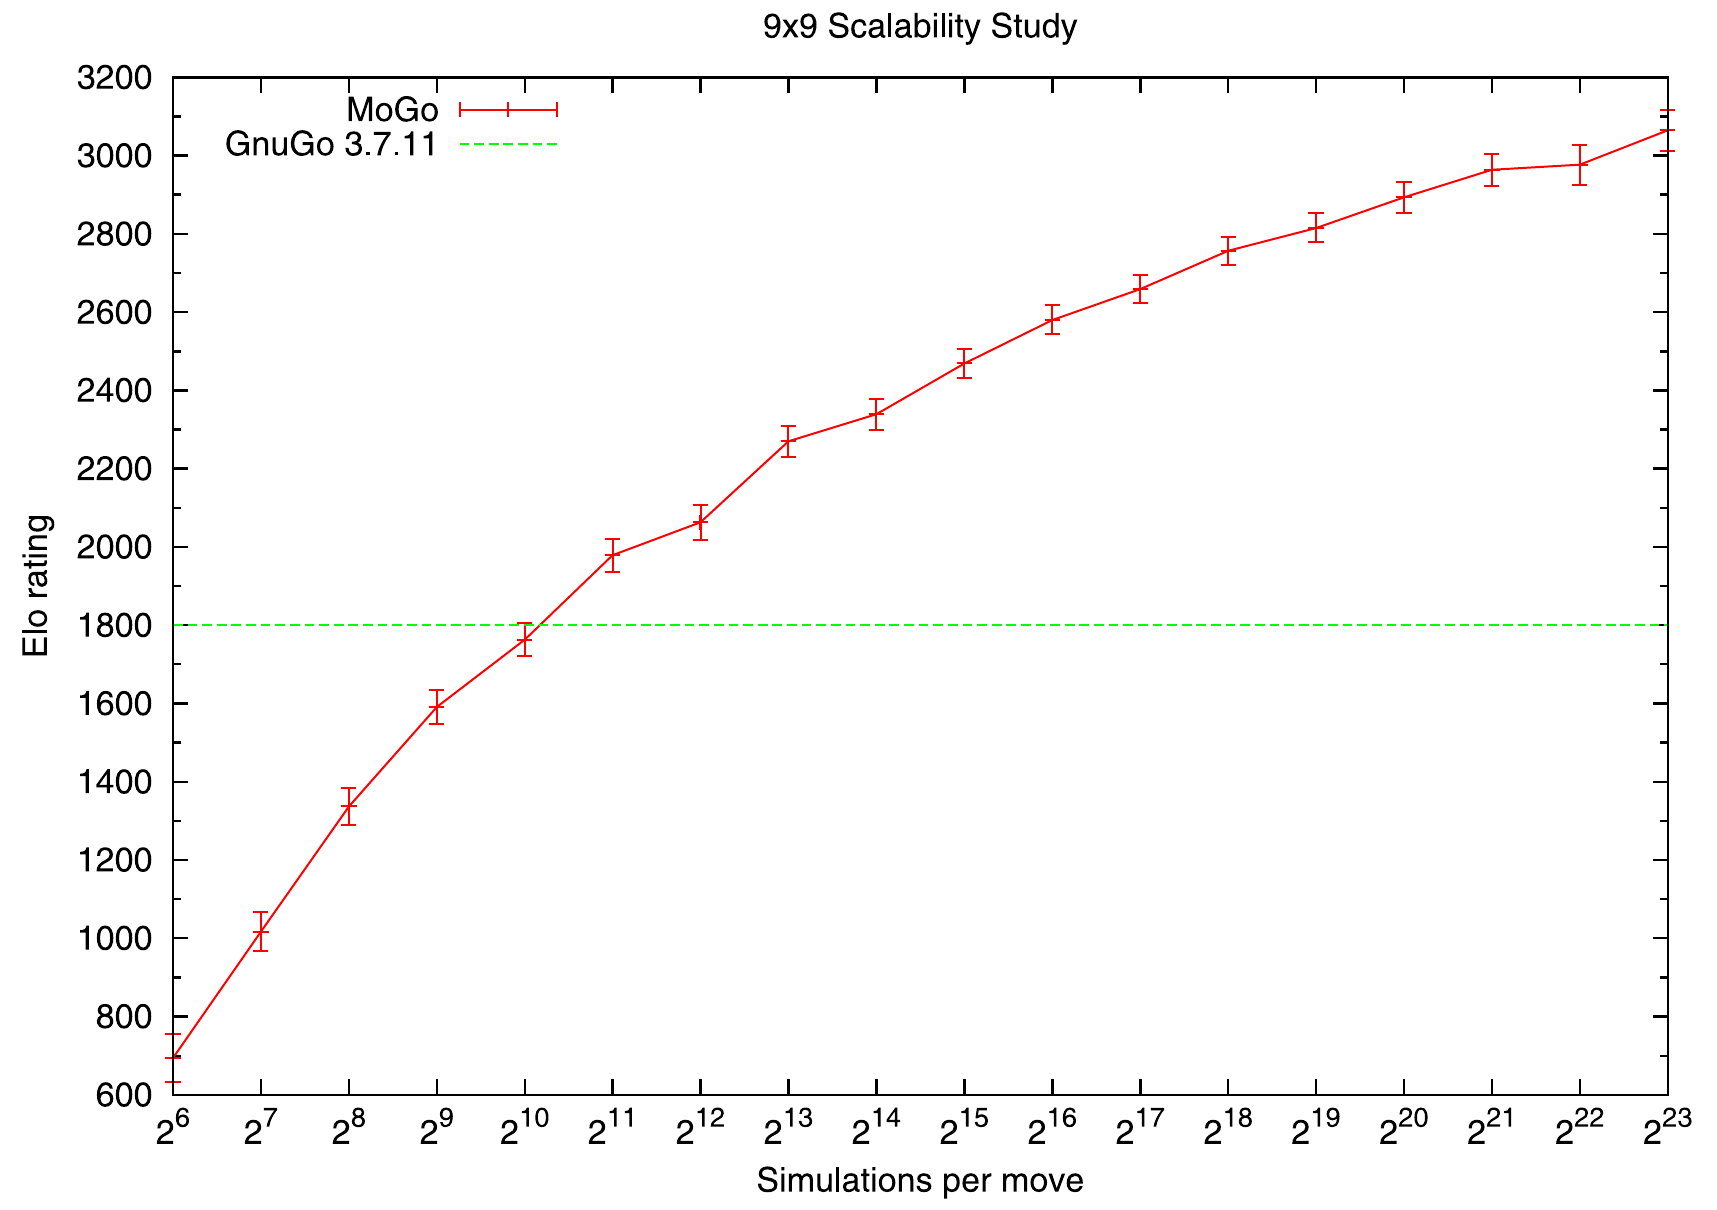
\includegraphics[height=7cm, keepaspectratio]{mogo_scaling.png}
    \caption{Elo rating of MoGo in relation to the computational resources granted to the algorithm \cite{gelly_monte-carlo_2011}}
    \label{mogo_scaling}
\end{figure}

\section{Learning agent}
The methods described until this point can be described as "Good old fashioned AI". They rely on search and human knowledge to perform adequately. We shift our focus now to methods that use learning mechanisms to improve their play. With MCTS we've actually seen a kind of intermediary form of algorithm as it is "simulating moves into the future, observing the outcome, and using the outcome to determine which moves are good ones is one kind of reinforcement learning." \cite{russell_artificial_2021}

\subsection{Reinforcement learning}
By devising a heuristic function, we basically told our agent what to do by indicating how a good position looks. The agent optimized its actions to be in a good position as described by the function. In reinforcement learning the agent learns what action to take through interaction. We don't predefine which actions are to be taken. The agent tries to discover which actions yield the best \textit{reward}. The numerical reward signal might come immediately, but e.g. in the case of Abalone the reward for actions taken comes much later by winning the game (or losing it). According to Sutton and Barto those are the key components of reinforcement learning: "trial-and-error search and delayed reward". \cite{sutton_reinforcement_2018}

Reinforcement learning is not a specific solution or method for this problem domain, all methods for "goal-directed agents interacting in an uncertain environment" are types of reinforcement learning. It is a general formalism that will help us reframe the problem of playing Abalone (well) in a new light.

\subsection{Markov decision process}
For reinforcement learning we also need to find a formalism for the environment. Originally derived as an extension of Markov Chains by Richard Bellman \cite{yang_markov_2019, bellman_markovian_1957}, the (finite) Markov Decision Process (MDP) describes sequential decision making where actions have long-term consequences, thus, effect future rewards. The MDP is an abstraction of "goal directed learning from abstraction" that reduces the problem to three signals of actions, states and rewards that are being exchanged between the agent and the environment. We already introduced the agent-environment interaction loop in figure \ref{agent_environment_loop}. We can reframe this image with the new terminology of the MDP framework in figure \ref{mdp_agent_environment}.

\begin{figure}
    \centering
    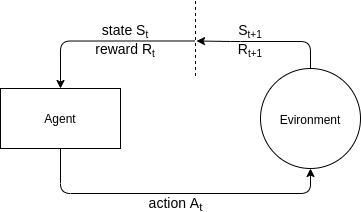
\includegraphics[height=4cm, keepaspectratio]{mdp_agent_environment.png}
    \caption{The markov decision process as agent-environment interaction loop}
    \label{mdp_agent_environment}
\end{figure}

We devide the passage of time into discrete timesteps $ t $ at which the agent senses the state $ S_t \in \mathcal{S} $ and then selects some action $ A_t \in \mathcal{A}(s) $. Resulting in that action is some reward $ R_{t+1} \in \mathcal{R} \subset \mathbb{R} $ that is recieved in the next timestep. For a \textit{finite} MDP the sets $ \mathcal{A}, \mathcal{S}$ and $ \mathcal{R} $ have a finite amount of elements.

The transitions between the state $ s $ and the next state $ s' $ is given by the function $ p $ which essentially defines the decision process as a whole:

$$
    p(s', r | s, a) \doteq Pr\{S_t=s', R_t = r | s_{t-1} = s, A_{t-1}=a\}
$$

As the random variables $ R_t $ and $ S_t $ only depend on the previous state and action, "the state must include information about all aspects of the past agent–environment interaction that make a difference for the future. If it does, then the state is said to have the \textit{Markov property}". \cite[p. 48]{sutton_reinforcement_2018}

From these properties of the MDP we can define the four central components of Reinforcement learning:

\paragraph{The reward signal} is the description of the agent's goal. A controller of a cooling system for a server farm might have the goal to minimize the energy spent for cooling while keeping the servers below a certain threshold. The reward signal then encompasses both of these subgoals. The controller has to maximize this reward. The \textit{reward hypothesis} states that:
\begin{quotation}
    That all of what we mean by goals and purposes can be well thought of as the maximization of the expected value of the cumulative sum of a received scalar signal (called reward).
\end{quotation}
Therefore, we introduce the reward $R_t $ and the goal $ G_t $ which is in the simplest case the sum of future rewards.

$$ G_t = R_{t+1} + R_{t+2} + ... + R_T $$

We might also discount the future rewards by some factor $\gamma \in [0, 1] $ to account for the decrease in certainty we have about future rewards:

$$ G_t = R_{t+1} + \gamma R_{t+2} + \gamma^2 R_{t+2} + ... = \sum_{k=0}^{\infty} \gamma^kR_{t+k+1}$$

\paragraph{The policy} is a mapping between the perceived states to probabilities for selecting each possible action. For TicTacToe we might imagine a table that lists for all possible states to the agent's action. Due to the size of the state  space \ref{complexity_table} in Abalone this would not be feasible, therefore we used search processes as a policy so far.

We denote the policy as the function $\pi $ defines a probability distribution over all actions $ a \in \mathcal{A}(s)$ for each $ s \in \mathcal{S} $. $ \pi(a|s)$ is probability at a given timestep $t$ for the action to be $ a = A_t $ under the condition that $ s = S_t $.

\paragraph{The value function} is an estimation of the reward for the agent to be in a given state $ s $.  As the reward for a state depends on what actions we take in the future, the value depends on the policy $ \pi $ defined above. Given that we are at timestep $ t $ and in state $ s = S_t $, the \textit{state-value function $v_{\pi}$}:

$$ v_{\pi}(s) = \mathbb{E}_{\pi}[G_t | S_t = s] = \mathbb{E}_{\pi}\left[\sum_{k=0}^{\infty} \gamma^kR_{t+k+1} \middle| S_t = s \right] $$

Furthermore, we define the value of action $a$ while being in state $s$ under the policy $pi$ as the \textit{action-value function} $q$:

$$ q_{\pi}(s) = \mathbb{E}_{\pi}[G_t | S_t = s, A_t = a] = \mathbb{E}_{\pi}\left[\sum_{k=0}^{\infty} \gamma^kR_{t+k+1} \middle| S_t = s, A_t = a \right] $$

\begin{figure}
    \centering
    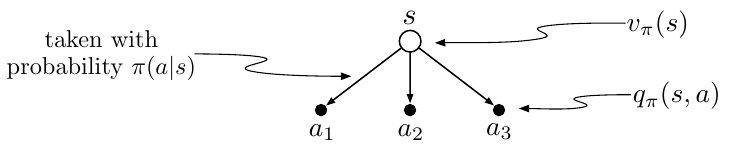
\includegraphics[height=2cm, keepaspectratio]{policy_value_action_value.png}
    \caption{A visual explanation of policy, value and action-value \cite[p.62]{sutton_reinforcement_2018}}
    \label{policy_value_action_value}
\end{figure}

The figure \ref{policy_value_action_value} shows how the three elements of policy, state-value and action-value relate to each other.

\paragraph{The model} helps to make predictions about how the environment might behave. For a given state and action it might return to the next state which aides in planning ahead. In the case of Abalone our model is the rules of the game, used by the function that returns all legal moves or the resulting board from a given board and a move.

The goal of reinforcement learning is to find (or approximate) a policy that maximzes the future reward for each action and state. For MDPs we define the \textit{optimal policy} for all $ s \in mathcal{S} $ by:

$$ v_{*}(s) \doteq \max_{\pi} v_{\pi}(s) $$

For this optimal policy we also have an optimal action-value function $ q_{*} $ for all $ s \in \mathcal{S}$:

$$ q_{*}(s, a) = \max_{\pi}q_{\pi}(s, a) $$

\subsection{Exploration vs. Exploitation}
\label{exploration_vs_exploitation}
As the agent builds its knowledge while it is engaged in the in the environment it has to weigh \textit{exploiting} the gathered knowledge for ensuring a safe short term reward or sacrificing it for \textit{exploring} other actions that might turn out to bring higher rewards in the future. To illustrate this fundamental tradeoff in reinforcement learning, let us imagine a gambling machine with 10 levers, a 10-armed bandit. At each timestep $ t $ we have to decide which lever to pull and then we recieve some reward $ R_t $. Each lever has some stationary distribution over the rewards, that is hidden from us. The distribution looks the the one given in figure \ref{10_armed_bandit}.

\begin{figure}
    \centering
    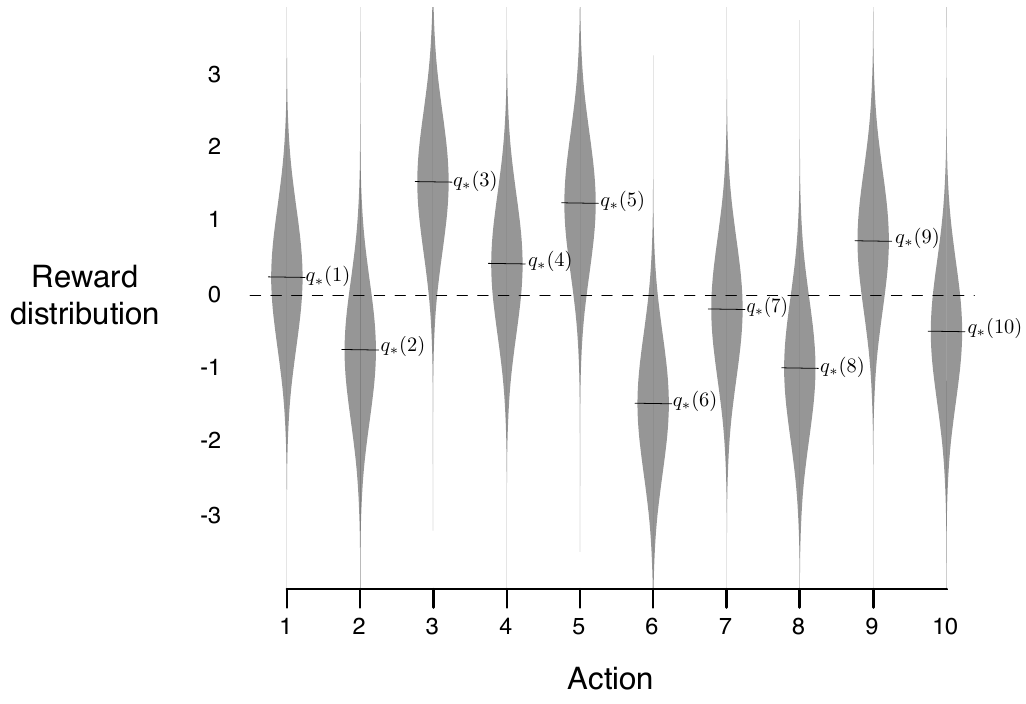
\includegraphics[height=7cm, keepaspectratio]{10_armed_bandit.png}
    \caption{The reward distributions of a 10-armed bandit \cite[p.28]{sutton_reinforcement_2018}}
    \label{10_armed_bandit}
\end{figure}

To estimate the action-value of each lever, we sum the rewards recieved for that lever $ R_t(a) $ and devide it by the number of times we've chosen the lever $ N_t(a) $ at the timestep $ t $.

$$
    Q_t(a) \doteq \frac{R_t(a)}{N_t{a}}
$$

This is called the \textit{sample-average} method. The simplest policy would be to just always choose the $ Q_t $ with the largest value.

$$
    A_t \doteq \operatorname*{argmmax}_a Q_t(a)
$$

Initially, we might choose a random lever and that yields a reward of 0. As all $ Q_t $ are still equivalent we choose another random lever giving us a reward of 1. Then ,according to the greedy policy, we just repeatedly pull this lever indefinitely. We just get stuck on exploiting the small knowledge we have gained. To allow for some exploration of other actions we introduce a small probability $\epsilon $ of choosing a different (random) action:
$$
    A_t =
    \begin{cases}
        \text{greedy } a & p = 1 - \epsilon \\
        \text{other } a  & p = \epsilon     \\
    \end{cases}
$$

If we continue for an infinite number of times $ Q_t $ is guaranteed to converge to $ q_{*} $ as we sample each action enough to estimate its stationary distribution. We might also let the $ \epsilon $ decay over time to ensure we exploit the optimal lever eventually. This shows how we have to carefully consider what knowledge we have and how we plan to expand it further.

\subsection{(Deep) Neural networks}

\paragraph{Loss functions}

\paragraph{(Stochastic) gradient descent}

\subsection{Deep reinforcement learning}

\subsection{AlphaGo and AlphaZero}
Now we have reached the culmination of our theoretical analysis. All the components we introduced so far constitute the knowledge necessary to understand AlphaGo and AlphaZero.



